%----------------------------------------------------------------------------------------
%	PACKAGES AND THEMES
%----------------------------------------------------------------------------------------
\documentclass[aspectratio=169,xcolor=dvipsnames]{beamer}
\usetheme{Simple}

\usepackage{hyperref}
\usepackage{graphicx} % Allows including images
\usepackage{booktabs} % Allows the use of \toprule, \midrule and \bottomrule in tables
\usepackage{graphicx}
\usepackage{amsmath}

\usepackage{mathtools}% superior to amsmath
\usepackage{tikz}
\usepackage{animate}

\makeatletter
\newcommand\mathcircled[1]{%
  \mathpalette\@mathcircled{#1}%
}
\newcommand\@mathcircled[2]{%
  \tikz[baseline=(math.base)] \node[draw,circle,inner sep=15pt] (math) {$\m@th#1#2$};%
}
\makeatother
%----------------------------------------------------------------------------------------
%	TITLE PAGE
%----------------------------------------------------------------------------------------

% The title
\title[short title]{Convolutional Neural Network}
\subtitle{Lecture 14}

\author[Narek Maloyan] {Narek Maloyan}
\institute[NTU] % Your institution may be shorthand to save space
{
    % Your institution for the title page
    Faculty of Computational Mathematics and Cybernetics \\
    Lomonosov Moscow State University
    \vskip 3pt
}
\date{\today} % Date, can be changed to a custom date


%----------------------------------------------------------------------------------------
%	PRESENTATION SLIDES
%----------------------------------------------------------------------------------------

\begin{document}

\begin{frame}
    % Print the title page as the first slide
    \titlepage
\end{frame}

\begin{frame}{Overview}
    % Throughout your presentation, if you choose to use \section{} and \subsection{} commands, these will automatically be printed on this slide as an overview of your presentation
    \tableofcontents
\end{frame}

%------------------------------------------------
\section{Pre deep learning era}
%------------------------------------------------

\begin{frame}{CV is hard}
    \begin{center}
        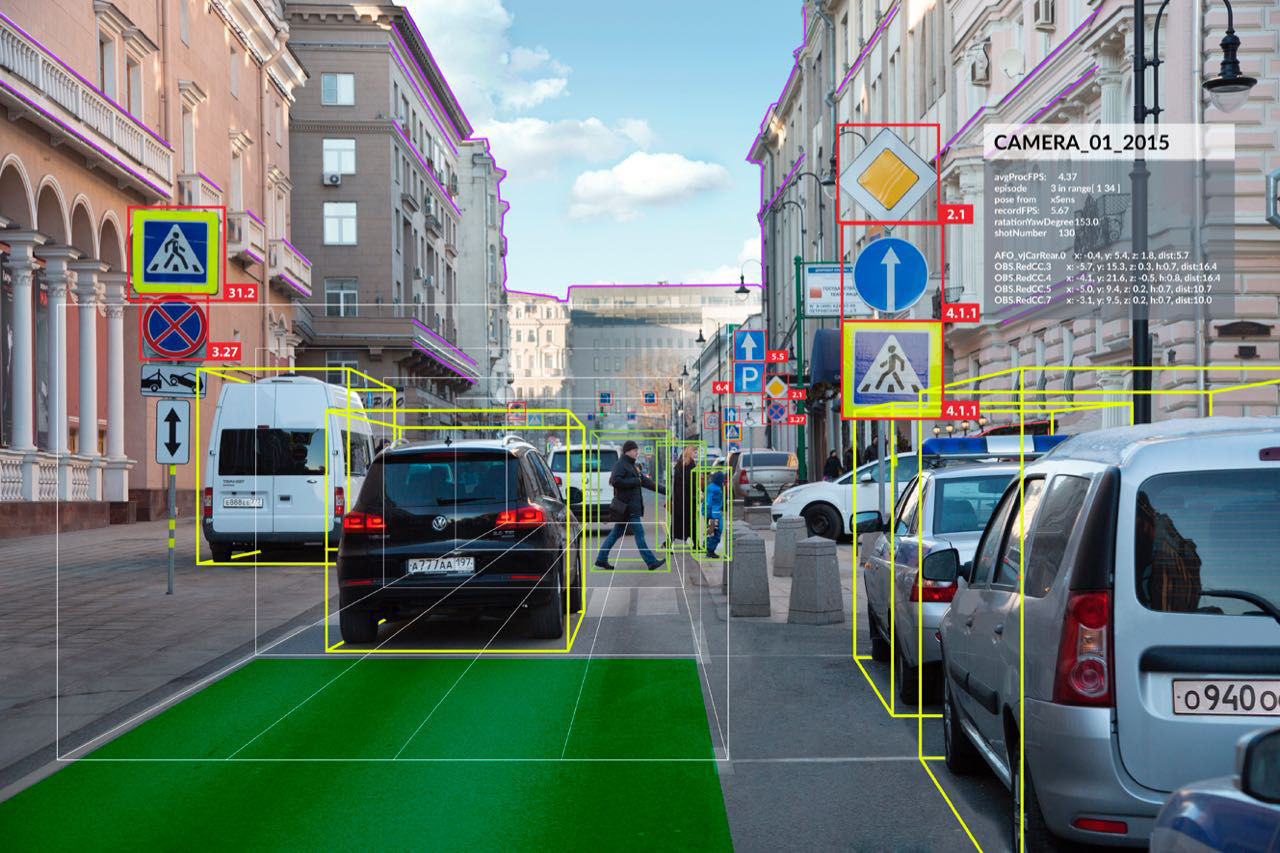
\includegraphics[width=\textheight]{../images/moscow.jpeg}
    \end{center}
\end{frame}

\begin{frame}{Applications}
    \begin{center}
        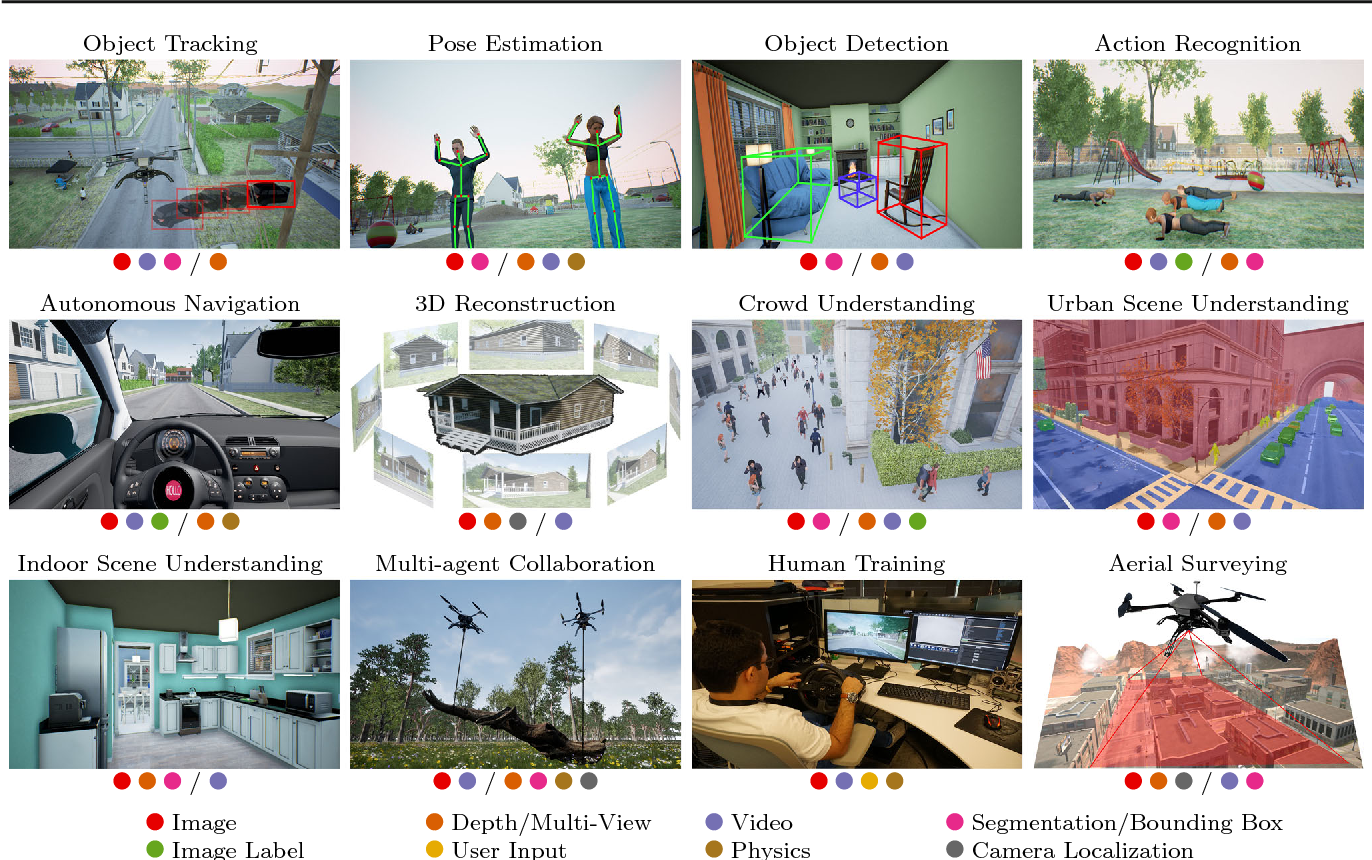
\includegraphics[width=1.3\textheight]{../images/cv-applications.png}
    \end{center}
\end{frame}

\begin{frame}{Feature extraction}
    \begin{center}
        \animategraphics[loop,controls,width=0.5\textheight]{10}{../images/face_mesh_andriod_gpu-}{0}{74}
    \end{center}
\end{frame}

\begin{frame}{Images as numbers}
    \begin{center}
        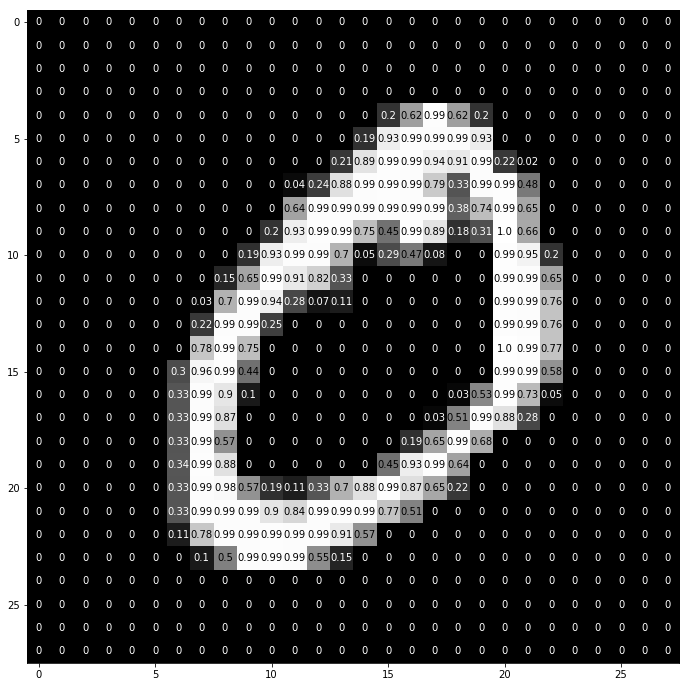
\includegraphics[width=0.8\textheight]{../images/mnist_cnn_keras_8_0.png}
    \end{center}
\end{frame}

\begin{frame}{CV pipeline}
    \begin{center}
        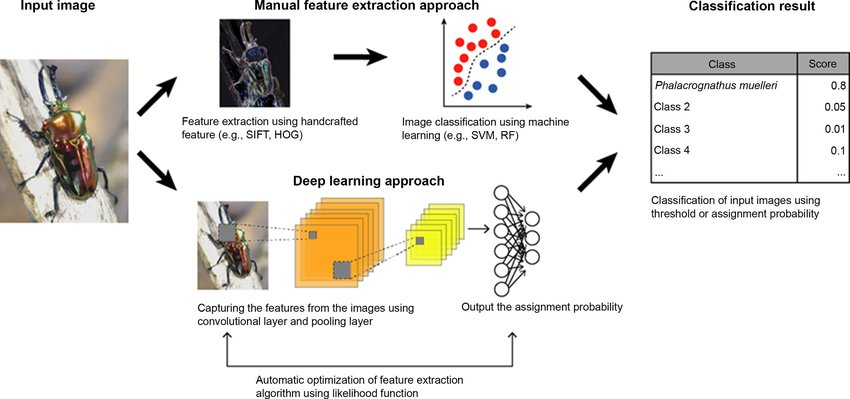
\includegraphics[width=\textwidth]{../images/Schematic-diagram-of-computer-vision-machine-learning-pipeline-for-image-based-species.png}
    \end{center}
\end{frame}

\begin{frame}{Variations}
    \begin{center}
        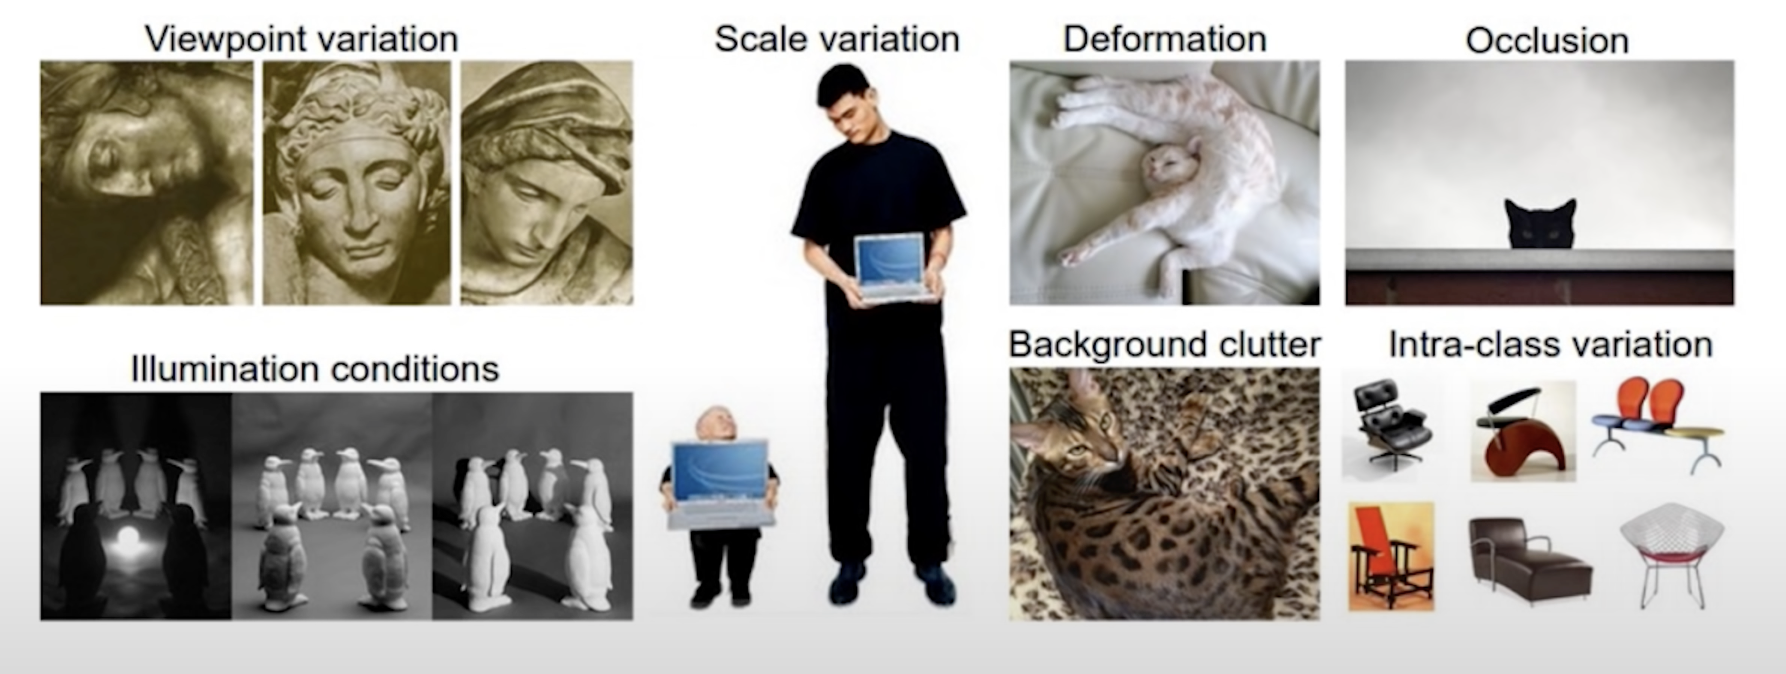
\includegraphics[width=\textwidth]{../images/variations.png}
    \end{center}
\end{frame}

\begin{frame}{Hierarchy of features}
    \begin{center}
        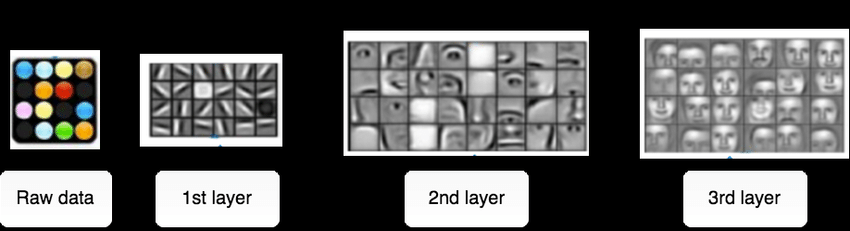
\includegraphics[width=\textwidth]{../images/hierarchy.png}
    \end{center}
\end{frame}
\end{document}